\documentclass{../../ece-report}

\usepackage{subcaption}
\usepackage{multirow}


\memostudent{Ty Davis}
\memotitle{Lab 8 - BJT DC Performance}
\memocourse{ECE 3110}
\memodate{\today}


\newcommand{\Vsub}[1]{\ensuremath{\textnormal{V}_{#1}}}
\newcommand{\sub}[2]{\ensuremath{\textnormal{#1}_{#2}}}

\renewcommand{\half}{\frac{1}{2}}



\begin{document}

\maketitle

\section{Introduction and Theory}

In this lab we are analyzing the performance of a BJT
transistor when supplied with DC voltages. Our goal
is to find the I-V curve that is produced. Fig.~\ref{fig:circuit}
shows the circuit that we are building in this lab.
We are going to control the voltages $V_{BE}$ and $V_{CE}$
to analyze the performance of the device.

\begin{figure}[h!]
  \centering
  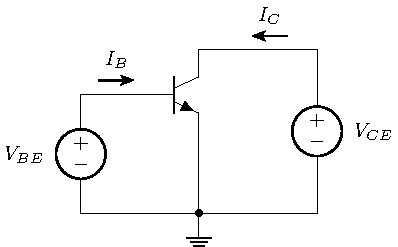
\includegraphics[width=0.5\textwidth]{../circuits/circuit.pdf}
  \caption{The BJT circuit we use in this lab.}
  \label{fig:circuit}
\end{figure}

\section{Simulation}

\subsection*{$I_C$ vs $V_{BE}$}

After building the circuit in the Multisim, we selected
the DC sweep measurement mode on the voltage source
$V_{BE}$. $V_{CE}$ is held constant at 5~V. Sweeping
$V_{BE}$ from 0 to 0.8 volts and measuring the current
$I_C$ resulted in the graph shown in Fig.~\ref{plot:sim_ic_vbe}.


Calculating $\beta$ is straight forward. We calculated $\beta = I_C / I_B$ at 
$V_{BE} = 0.7~\si{\V}$. The result is $\beta = 161.207$.

\begin{figure}[h!]
  \centering
  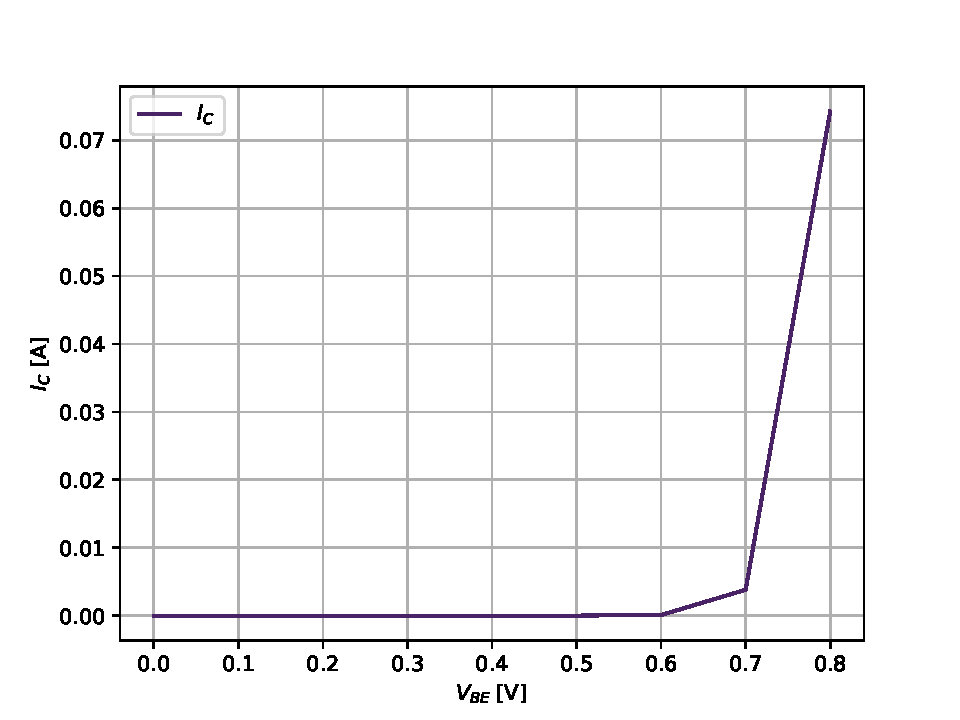
\includegraphics[width=0.6\textwidth]{../plots/pdf/sim_sweep_vbe.pdf}
  \caption{$I_C$ vs $V_{BE}$ simulation results.}
  \label{plot:sim_ic_vbe}
\end{figure}

\subsection*{$I_C$ vs $V_{CE}$}

For this simulation, we measured the current $I_C$ in
response to a DC sweep of $V_{CE}$ after setting the
voltage $V_{BE}$ to 3 different voltages, as shown in
Fig.~\ref{plot:sim_ic_vce}. As you can see, with $V_{BE}$ set to 
just 0.6~V, the device was never activated and current would
never flow through $I_C$. However, when $V_{BE}$ was set to a 
higher voltage, it activates the device and allows the current
to flow. 

\begin{figure}[h!]
  \centering
  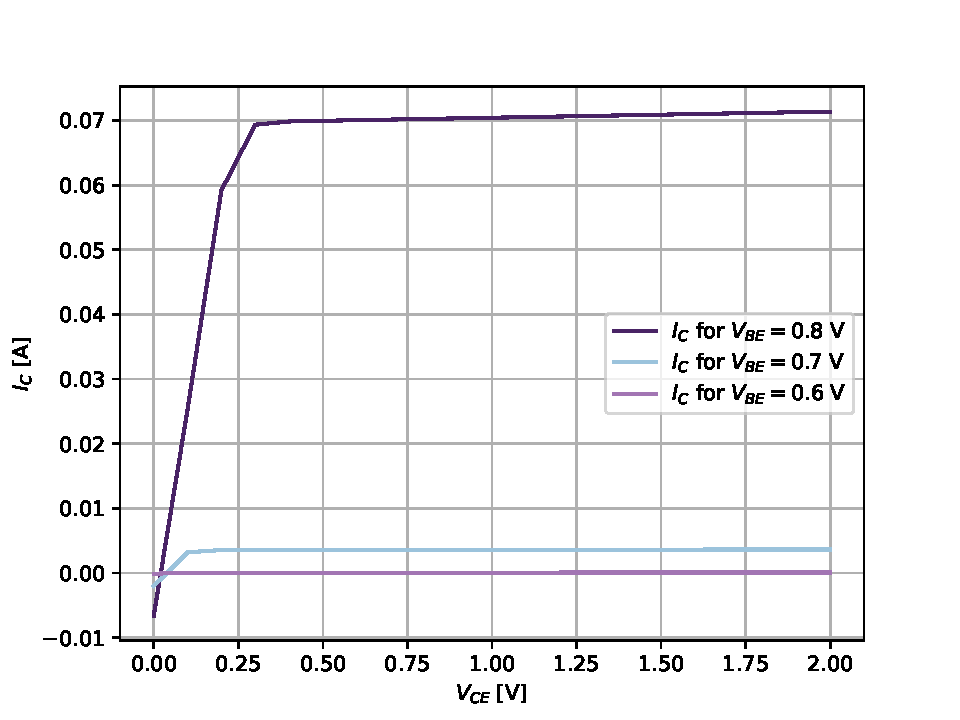
\includegraphics[width=0.6\textwidth]{../plots/pdf/sim_sweep_vce.pdf}
  \caption{$I_C$ vs $V_{CE}$ simulation results.}
  \label{plot:sim_ic_vce}
\end{figure}

\section{Results}

After simulating the performance of the device, we built the circuit
to measure and compare the results. 

\subsection*{$I_C$ vs $V_{BE}$}

Similar to the simulation, we swept $V_{BE}$ from 0 to 0.8~V, while keeping
$V_{CE}$ at a constant 5~V. Fig.~\ref{plot:meas_ic_vbe} shows the results,
and they look very similar to the simulation results.

Calculating $\beta$ was similar to the simulation calculation.
We found that $\beta = 18.3~\si{\mA} / 398~\si{\uA} = 45.98$.

\begin{figure}[h!]
  \centering
  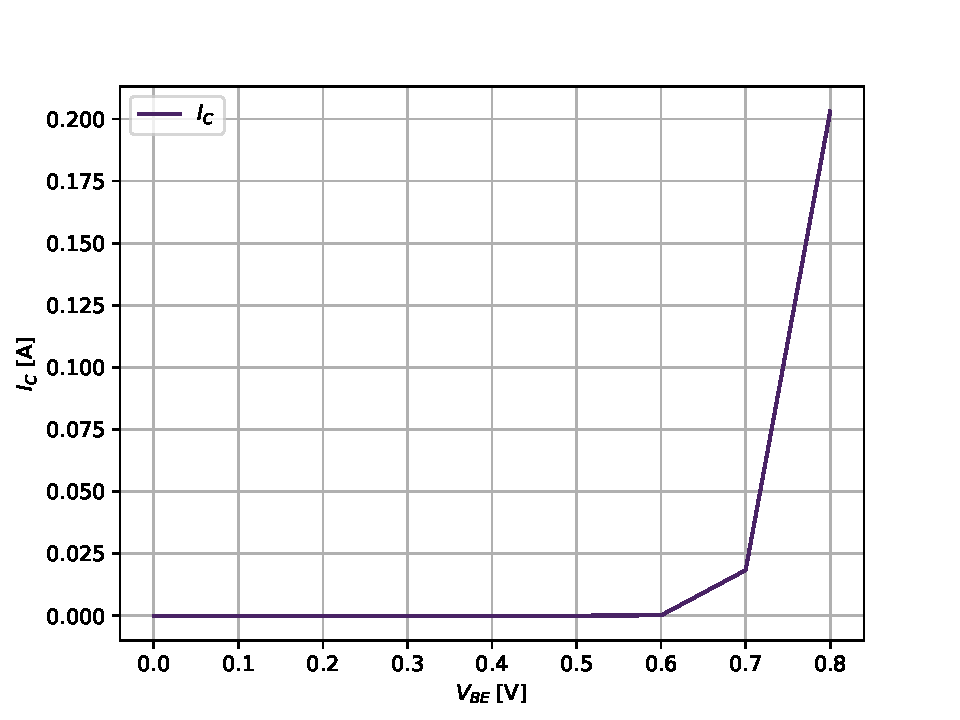
\includegraphics[width=0.6\textwidth]{../plots/pdf/meas_sweep_vbe.pdf}
  \caption{$I_C$ vs $V_{BE}$ measurement results.}
  \label{plot:meas_ic_vbe}
\end{figure}

\subsection*{$I_C$ vs $V_{CE}$}

Lastly, we swept $V_{CE}$ after setting $V_{BE}$ to each 0.6, 0.7, and 0.8~V.
The resulting graph is shown in Fig.~\ref{plot:meas_ic_vce}.


\begin{figure}[h!]
  \centering
  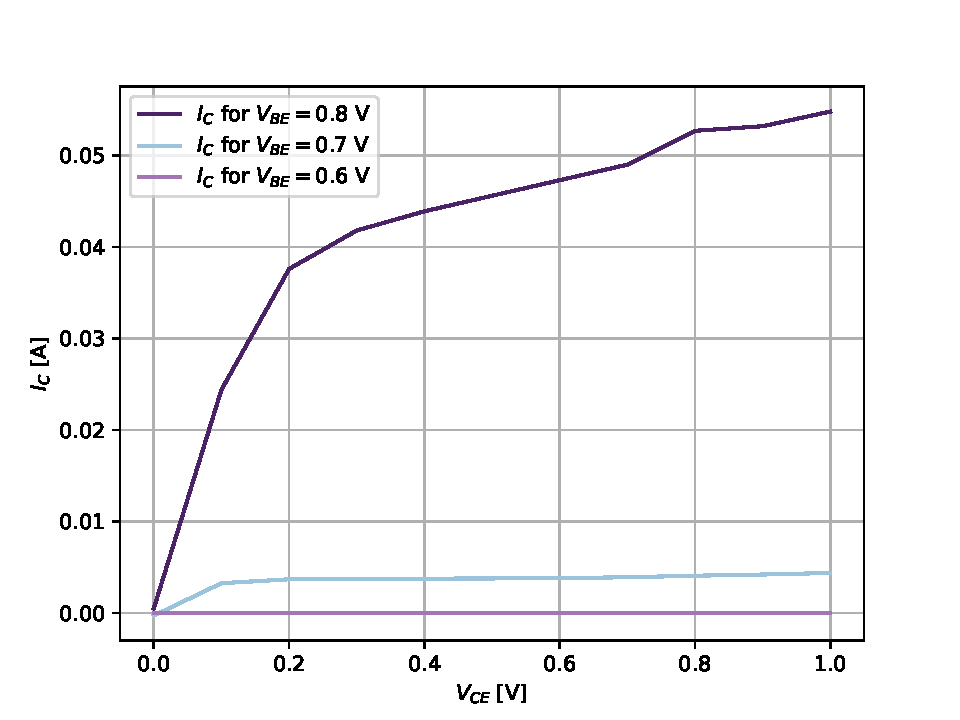
\includegraphics[width=0.6\textwidth]{../plots/pdf/meas_sweep_vce.pdf}
  \caption{$I_C$ vs $V_{CE}$ measurement results.}
  \label{plot:meas_ic_vce}
\end{figure}

\section{Post-Measurement Exercise}

The main difference between the simulation and measurement
results is that the current was much higher in our measurements
as compared to the simulation. Compare Figs.~\ref{plot:sim_ic_vbe}
and \ref{plot:meas_ic_vbe} and see that at $V_{BE} = 0.8~\si{\V}$,
the current through the BJT is at $\approx 200~\si{\mA}$ in the real
circuit and only $\approx 70~\si{\mA}$ in the simulation. Such a high
current did cause the BJT to heat up considerably. 

With high temperatures at that voltage, the $I_C$ vs
$V_{CE}$ graph seemed affected in the real circuit.
The current wasn't ever able to settle when we were
measuring it, and it never appeared to truly reach active
region, but the current did stop increasing exponentially.

\subsection*{Early Voltage}

Calculating the Early Voltage from the simulation was
a matter of calculating the slope from the simulation curves
once they reach active region and finding the point where $I_C$ 
would equal 0~A. The average Early Voltage that we calculated
from the simulation was found to be -65.5~V.

The Early Voltage was not calculated for $V_{BE} = 0.6~\si{\V}$,
because the voltage was always zero and it never reached
the active region of operation.

The difference between the remaining two $V_A$ calculations was
15.4~V, so while they were within the same order of magnitude, they
weren't necessarily the exact same value.

\end{document}
